\documentclass[11pt, oneside]{article}   	% use "amsart" instead of "article" for AMSLaTeX format
\usepackage{geometry}                		% See geometry.pdf to learn the layout options. There are lots.
\geometry{letterpaper}                   		% ... or a4paper or a5paper or ... 
%\geometry{landscape}                		% Activate for for rotated page geometry
%\usepackage[parfill]{parskip}    		% Activate to begin paragraphs with an empty line rather than an indent
\usepackage{graphicx}				% Use pdf, png, jpg, or eps� with pdflatex; use eps in DVI mode
								% TeX will automatically convert eps --> pdf in pdflatex		
\usepackage{amssymb}
\usepackage{amsmath}
\usepackage{parskip}

\title{Law of Cosines and the Dot Product}
%\author{The Author}
%\section{}
% \subsection*{R code}
\date{}							% Activate to display a given date or no date

\graphicspath{{/Users/telliott_admin/Dropbox/Tex/png/}}

\begin{document}
\maketitle
\Large
\noindent

The law of cosines relates the length of any two sides of a triangle and the angle they form with each other, to the magnitude of the side opposite.  Consider this figure:

\begin{center} 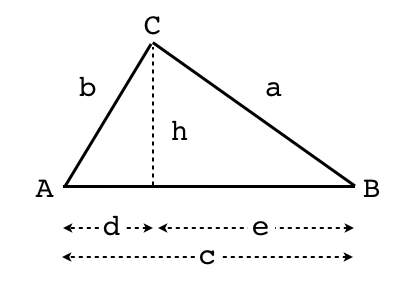
\includegraphics [scale=0.5] {Triangle.png} \end{center}

The law of cosines states that
\[ a^2 = b^2 + c^2 - 2bc \cos A \]

In the case where $A = 90$ degrees, $\cos A = 0$, and this reduces to Pythagoras' statement about right triangles.  We can prove the law pretty easily by fooling around with the two right triangles formed using the height $h$.  We divide $c$ into $d + e$, and Pythagoras says that
\[ b^2 = d^2 + h^2 \]
\[ a^2 = e^2 + h^2 = (c-d)^2 + h^2 \]

Eliminate $h$ by combining the two statements:
\[ a^2 = (c-d)^2 + b^2 - d^2 \]
\[ = c^2 - 2cd + d^2 + b^2 - d^2 \]
\[ = c^2 - 2cd + b^2 \]

We must be making progress since $d^2$ is gone.  Now we just need to involve the cosine of $A$ (and eliminate $d$) so we notice that
\[ \frac{d}{b} = \cos A \]
\[ d = b \cos A \]

so
\[ a^2 = c^2 - 2cb \cos A + b^2 \]

rearrange that to give the law as stated above.

In vector analysis we encounter the dot product.  One formulation is that 
\[ \mathbf{u} \cdot \mathbf{v} = uv \cos \theta \]

for any two vectors $\mathbf{u}$ and $\mathbf{u}$, where $\theta$ is the angle between the two vectors and their magnitudes are $u$ and $v$.  And again, we invoke Pythagoras to arrive at the very useful statement that
\[ \mathbf{u} \cdot \mathbf{v} = 0 \iff \theta = \frac{\pi}{2} \]

Two vectors are orthogonal or perpendicular if, and only if, their dot product is zero.  

In order to prove this we will show that the law of cosines and this statement are equivalent.  We first equate $\mathbf{u}$ with the vector extending from $A$ to $B$ in the figure, and similarly $\mathbf{v}$ will be the vector extending from $A$ to $C$.

\begin{center} 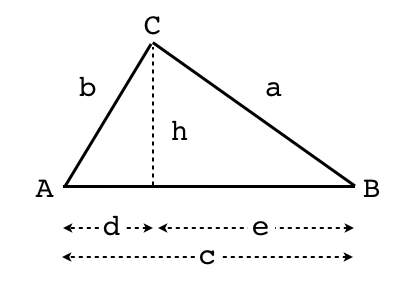
\includegraphics [scale=0.5] {Triangle.png} \end{center}
Going back to the law of cosines, which we proved above:
\[ a^2 = b^2 + c^2 - 2cb \cos A \]

The side that we called $c$ is now $\mathbf{u}$, and its length squared is:
\[ c^2 = |\mathbf{u}|^2 =  \mathbf{u} \cdot \mathbf{u} \]

Similarly
\[ b^2 =  \mathbf{v} \cdot \mathbf{v} \]

Realize that the vector from $B$ to $C$, when added to $\mathbf{u}$, equals $\mathbf{v}$.  Thus side $a$ corresponds to $\mathbf{v} - \mathbf{u}$ and so
\[ a^2 = (\mathbf{v} - \mathbf{u}) \cdot  (\mathbf{v} - \mathbf{u})  \]

Now write the law of cosines in terms of vectors (with the angle $A$ becoming $\theta$):
\[ a^2 = b^2 + c^2 - 2cb \cos A \]
is the same as
\[ (\mathbf{v} - \mathbf{u}) \cdot  (\mathbf{v} - \mathbf{u}) = \mathbf{v} \cdot \mathbf{v} + \mathbf{u} \cdot \mathbf{u} - 2cb \cos \theta \]

The dot product is distributive over addition and subtraction (working an example with components should convince you), so 
\[ (\mathbf{v} - \mathbf{u}) \cdot  (\mathbf{v} - \mathbf{u}) = \mathbf{v} \cdot \mathbf{v} - 2 \ \mathbf{v} \cdot \mathbf{u} + \mathbf{u} \cdot \mathbf{u}  \]

Equating the two expressions we obtain
\[  \mathbf{v} \cdot \mathbf{v} + \mathbf{u} \cdot \mathbf{u} - 2cb \cos \theta = \mathbf{v} \cdot \mathbf{v} - 2 \ \mathbf{v} \cdot \mathbf{u} + \mathbf{u} \cdot \mathbf{u}  \]

Canceling
\[ - 2cb \cos \theta = - 2 \ \mathbf{v} \cdot \mathbf{u}   \]

and canceling some more
\[ cb \cos \theta =  \mathbf{v} \cdot \mathbf{u}   \]

But $c = |\mathbf{u}| = u $ and $b = |\mathbf{v}| = v $ so we have finally
\[ |\mathbf{u}|  |\mathbf{v}| \cos \theta = u  v \cos \theta =  \mathbf{v} \cdot \mathbf{u} =  \mathbf{u} \cdot \mathbf{v}  \]

(The last step is by commutativity of the dot product), so 

\[ \mathbf{u} \cdot \mathbf{v}  =  u  v \cos \theta \]

which is what we wanted to prove.

\end{document}  